\documentclass[runningheads,a4paper]{llncs}

\usepackage[american]{babel}

\usepackage{graphicx}

%extended enumerate, such as \begin{compactenum}
\usepackage{paralist}

%put figures inside a text
%\usepackage{picins}
%use
%\piccaptioninside
%\piccaption{...}
%\parpic[r]{\includegraphics ...}
%Text...

%Sorts the citations in the brackets
%\usepackage{cite}

%for easy quotations: \enquote{text}
\usepackage{csquotes}

\usepackage[T1]{fontenc}

%enable margin kerning
\usepackage{microtype}

%better font, similar to the default springer font
\usepackage[%
rm={oldstyle=false,proportional=true},%
sf={oldstyle=false,proportional=true},%
tt={oldstyle=false,proportional=true,variable=true},%
qt=false%
]{cfr-lm}
%
%if more space is needed, exchange cfr-lm by mathptmx
%\usepackage{mathptmx}

%for demonstration purposes only
\usepackage[math]{blindtext}

\usepackage[
%pdfauthor={},
%pdfsubject={},
%pdftitle={},
%pdfkeywords={},
bookmarks=false,
breaklinks=true,
colorlinks=true,
linkcolor=black,
citecolor=black,
urlcolor=black,
%pdfstartpage=19,
pdfpagelayout=SinglePage
]{hyperref}
%enables correct jumping to figures when referencing
\usepackage[all]{hypcap}

\usepackage[capitalise,nameinlink]{cleveref}
%Nice formats for \cref
\crefname{section}{Sect.}{Sect.}
\Crefname{section}{Section}{Sections}
\crefname{figure}{Fig.}{Fig.}
\Crefname{figure}{Figure}{Figures}

\usepackage{xspace}
%\newcommand{\eg}{e.\,g.\xspace}
%\newcommand{\ie}{i.\,e.\xspace}
\newcommand{\eg}{e.\,g.,\ }
\newcommand{\ie}{i.\,e.,\ }

%introduce \powerset - hint by http://matheplanet.com/matheplanet/nuke/html/viewtopic.php?topic=136492&post_id=997377
\DeclareFontFamily{U}{MnSymbolC}{}
\DeclareSymbolFont{MnSyC}{U}{MnSymbolC}{m}{n}
\DeclareFontShape{U}{MnSymbolC}{m}{n}{
    <-6>  MnSymbolC5
   <6-7>  MnSymbolC6
   <7-8>  MnSymbolC7
   <8-9>  MnSymbolC8
   <9-10> MnSymbolC9
  <10-12> MnSymbolC10
  <12->   MnSymbolC12%
}{}
\DeclareMathSymbol{\powerset}{\mathord}{MnSyC}{180}

%improve wrapping of URLs - hint by http://tex.stackexchange.com/a/10419/9075
\makeatletter
\g@addto@macro{\UrlBreaks}{\UrlOrds}
\makeatother

% correct bad hyphenation here
\hyphenation{op-tical net-works semi-conduc-tor}

\begin{document}

%Works on MiKTeX only
%hint by http://goemonx.blogspot.de/2012/01/pdflatex-ligaturen-und-copynpaste.html
%also http://tex.stackexchange.com/questions/4397/make-ligatures-in-linux-libertine-copyable-and-searchable
%This allows a copy'n'paste of the text from the paper
\input glyphtounicode.tex
\pdfgentounicode=1

\title{Big Data with High Performance Computing (HPC)}
%If Title is too long, use \titlerunning
%\titlerunning{Short Title}

%Single insitute
\author{Tarek El-Ghazawi \and Krunal Puri \and Armin Mehrabian}
%If there are too many authors, use \authorrunning
%\authorrunning{First Author et al.}
\institute{George Washington University}

%Multiple insitutes
%Currently disabled
%
\iffalse
%Multiple institutes are typeset as follows:
\author{Tarek El-Ghazawi\inst{1} \and Krunal Puri\inst{1} \and Armin Mehrabian \inst{1} }
%If there are too many authors, use \authorrunning
%\authorrunning{First Author et al.}

\institute{
George Washington University\\
\email{...}\and
Insitute 2\\
\email{...}
}
\fi
			
\maketitle

\begin{abstract}
Abstract goes here
\end{abstract}

\keywords{...}

%%%%%%%%%%%%%%%%%%%%%%%%%%%%%%%%%%%%%%%%%%%%%%%%%%%%%%%%%%%%%%%%%%%%%%%%%%%%%%%
\section{Introduction}\label{sec:intro}
%%%%%%%%%%%%%%%%%%%%%%%%%%%%%%%%%%%%%%%%%%%%%%%%%%%%%%%%%%%%%%%%%%%%%%%%%%%%%%%
%\blindtext
With the recent emergence of Big Data over the past few years, one of the questions that arises is, how Big Data is different from High Performance Computing (HPC) at various levels such as application, technology, investment, etc. Another critical question to be asked is if Big Data is widely different from HPC, which of the technologies may we want to adopt or, do we really have to choose one from the two to apply to our problems? Another scenario is that the gap between Big Data and HPC may form a spectrum of choices rather than two independent worlds. To answer these questions in this chapter we will first bring an introduction and look at Big Data and HPC from a high level abstraction view. Then, we explain the state of the art efforts to take advantage of the best of two worlds. Finally, we will address future challenges and future directions.\\

\begin{figure}
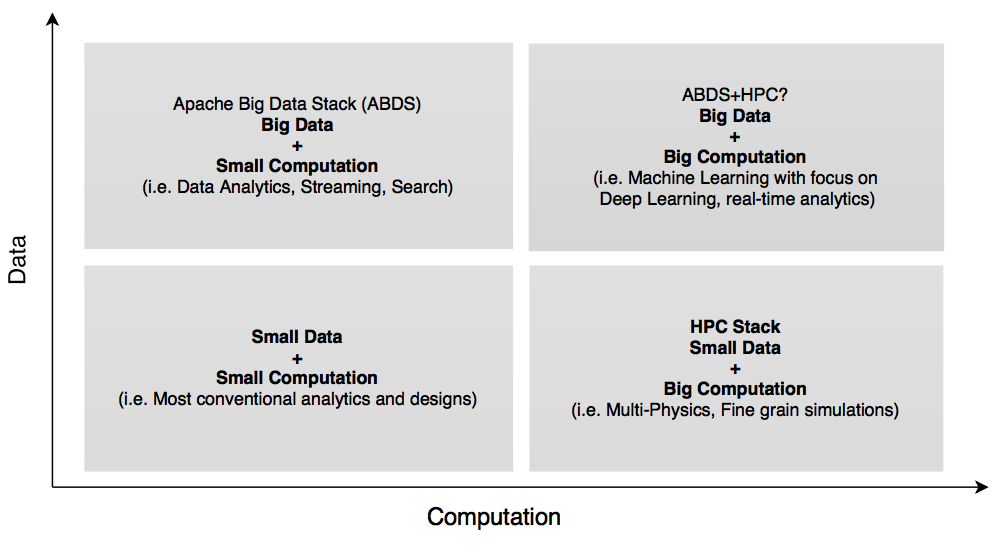
\includegraphics[scale=0.31]{./images/BigData_HPC.png}
\centering
\caption{Matrix of data and computation applications.}
\label{fig:bigdata_hpc_matrix}
\end{figure}
In order to answer the above questions we first may need to identify the workloads and computational requirements of workflows for our applications. It is also important to not focus only current trends, and take into account the future data and computation demands. Figure \ref{fig:bigdata_hpc_matrix} shows the matrix of data size versus computation size for some applications. It also shows that the current big data technologies, formed around Apache Big Data Stack (ABDS), is data-intensive but focused less on computational performance. On the other hand the High Performance Computing (HPC), which mostly applied to solving scientific problems, has been mostly concentrated on computation-savvy, data limited application such and iterative simulations.\\

Over the past decade, the rate of data generation has dramatically increased. As a result, we saw the emergence of data-intensive applications to solve a range of problems from data  distribution and management to data processing. The open-source Apache Big Data Stack with it's Hadoop Data File System (HDFS) kernel and many higher abstraction level frameworks for data analytics and machine learning has provided a coherent ecosystem, which has dominated the industry.\\

In contrast, HPC with roots in computational intensive scientific computing, has mainly been applied and fine-tuned for particular problems, which resulted in significantly more limited implementations compared to ABDS.
\begin{figure}
	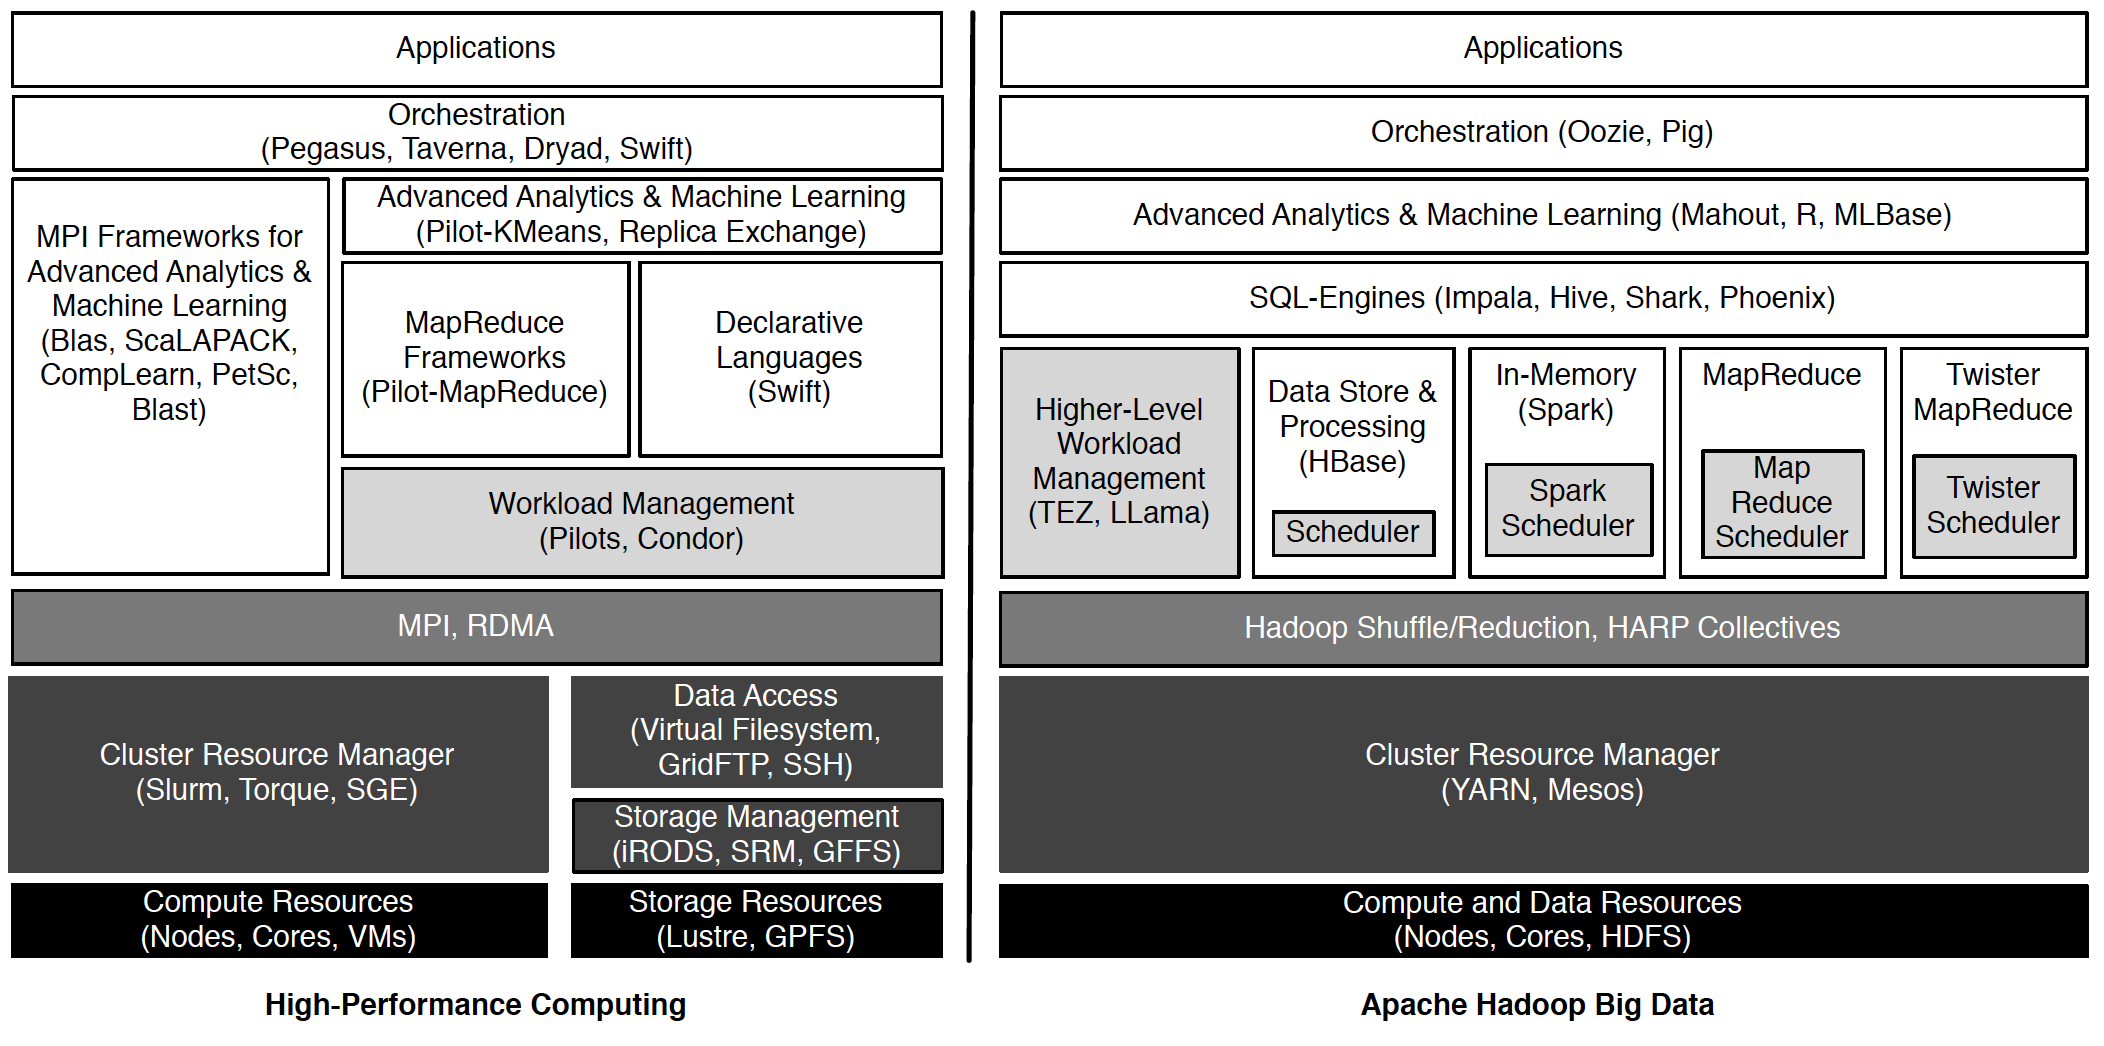
\includegraphics[scale=0.33]{./images/Ecosystems.png}
	\centering
	\caption{Apache Big Data Stack (ABDS) ecosystem vs. High Performance Computing (HPC) ecosystem \cite{Jha2014}.}
	\label{fig:bigdata_hpc_ecosystem}
\end{figure}
Figure \ref*{fig:bigdata_hpc_ecosystem} depicts the HPC and Big Data ecosystems from many abstraction level view. The lowest layers are the resources, resource management, and communication layers. The higher layers comprise of processing and analytical components. In remaining parts of this section we compare current typical HPC and Big Data architectures and their respective ecosystems.
\subsection{HPC Architecture}
A typical HPC architecture consists of processing units such a multi-core structures, possibly accelerated by GPUs, FPGAs, or even CPUs such as intel Xeon Phi. These processing units are supported by local storage units with Lustre \cite{braam2004lustre} or General Parallel File System (GPFS) \cite{FrankSchmuck} file system or a remote storage connected through a fast network such as Infiniband.\\

Lustre and GPFS are parallel file systems designed mainly for clusters. Lustre, which combines the words Linux and Cluster is generally accepted as the file system with scalability for large scale cluster computing. Due to its high performance it has been continuously used by top supercomputers. On the other hand GPFS introduced by IBM and adopted by many of the biggest companies all around the word. GPFS have it roots in academic grounds and its scalability is a matter of question. Storage resources in HPC are managed by storage management unit such as integrated Rule-Oriented Data-management System (iRODS), Storage Resource Manager interface (SRM) \cite{shaun2007storage} \cite{rajasekar2010irods},  Global Federated File System (GFFS) \cite{grimshaw2013gffs}.\\

While storage resources are usually shared in applications, computational resources are local. Such local compute resources are managed by their own management units such as Slurm \cite{yoo2003slurm}, Torque \cite{staples2006torque}, and Sun Grid Engine (SGE) \cite{gentzsch2001sun}.

In HPC applications, data need to fly around across network using a low latency communication. These fast interconnect networks along with features such as non-blocking and one-sided communications allow for more data-intensive HPC within HPC environment. As a matter of fact, data-intensive applications are not totally unfamiliar to HPC community. There has been many approaches to implement MapReduce compatible with HPC environment such as MapReduce-MPI \cite{plimpton2011mapreduce}, Pilot-MapReduce \cite{mantha2012pilot}, and Twister for machine learning applications \cite{ekanayake2010twister}.In a parallel effort, there has been many implementations of data intensive loosely coupled tasks at run-time level \cite{luckow2012p}\cite{raicu2008many}\cite{deelman2009workflows}.
\subsection{ABDS Architectures}
The Apache Big Data Stack is formed around the Hadoop Distributed File System (HDFS), which originated at Yahoo but is an open source implementation of Google's file system \cite{shvachko2010hadoop} \cite{ghemawat2003google}. As we know now, the idea behind ABDS was to bring the computation to data, which is usually stored at cheap commodity hardware. Hadoop 1.0 also took advantage of Google's MapReduce programming model for data processing. MapReduce imposes it's own limitations since all processes is forced to be implemented in the form of a mapper followed by a reducer. MapReduce's inherent limitations along with tight coupling of Hadoop and MapReduce proved to be inflexible when used in applications such as iterative computations, which is an indispensable piece of all Machine Learning algorithms.\\

As a result of such deficits in Hadoop 1.0, Apache YARN was introduced with Hadoop 2.0 as a much more lenient resource manager, enabling many applications and frameworks with higher level abstractions \cite{vavilapalli2013apache}. YARN's key feature was introduction multi-level scheduling, which would allow higher level applications to schedule their own processes. As a results we saw the emerge of many high level applications such as, HBase, a column based distributed database, Spark, Giraph, which are iterative and graph processing applications\cite{borthakur2011apache}\cite{zaharia2012resilient}.
\newpage
\section{State of the art projects}
In this section we will review some of the state of the art researches and projects within HPC-Big Data domains. We categorized these project under four class of research topics, namely,
\begin{enumerate}
	\item Integration of HPC and ABDS stack
	\item Machine Learning (ML) using HPC
	\item Parallel databases
	\item Parallel I/O
	
\end{enumerate}
\subsection{Integration of HPC and Big Data stack}
Big Data and HPC used to be used interchangeably for many years. But, with HPC targeting scientific problems with huge number of iterations, and Big Data aiming for relatively simple model on huge datasets, it seems they diverged for a while. As the rate of data generation increase, deployment of HPC tools and techniques seem more and more inevitable. Following projects are some of the state of the arts in combining HPC and Big Data stack.
\subsubsection{High Performance Big Data System (HPBDS) project \cite{qiu2014towards}}: The HPBDS project aims for integrating some of the components of the HPC such as scientific libraries, fast communication and resource management features with commercial Big Data ecosystem namely, ABDS.\\

The primary proposed execution of HPBDS is built around Apache Hadoop and therefore named High Performance Computing Big Data Stack (HPC-ABDS). The HPC-ABDS comprise two sub-project,
\begin{figure}[h]
	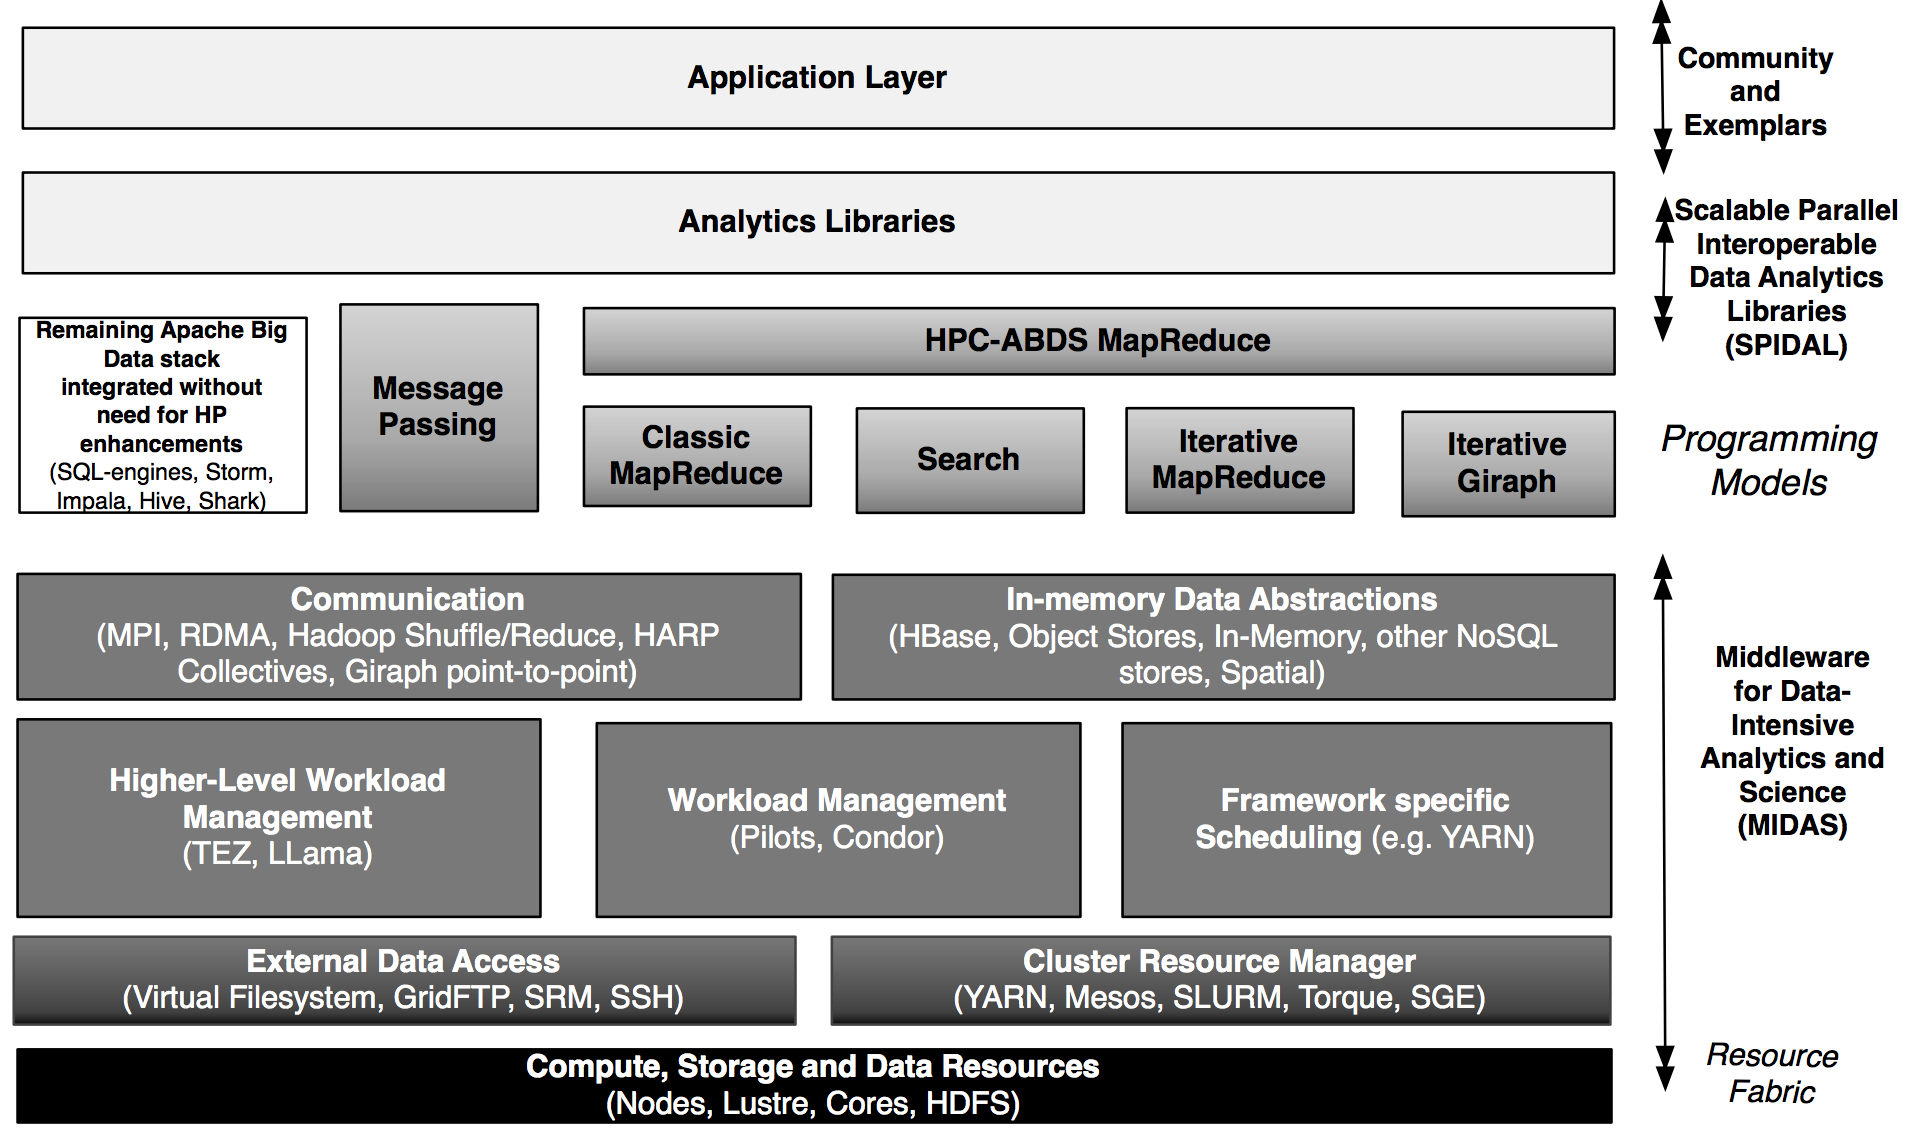
\includegraphics[scale=0.25]{./images/MIDASSPIDAL.png}
	\centering
	\caption{MIDAS and SPIDAL within HPC-ABDS stack\cite{qiu2014towards}}
	\label{fig:MIDAS_SPIDAL}
\end{figure}
\begin{enumerate}
	\item Middleware for Data Intensive Analytics and Science (MIDAS)
	\item Scalable Parallel Interoperable Data Analytics Library (SPIDAL)  
\end{enumerate}

Figure \ref{fig:MIDAS_SPIDAL} depicts the structure of the MIDAS-SPIDAL with trespect to the overall HPC-ABDS stack. MIDAS is proposed to provide a lower level infrastructure based on which higher level components such as libraries operates. On the other hand SPIDAL goal is to take advantage of useful tool within HPC such as MPI, PETSc, and SCALAPACK and modify them for data intensive applications.\\

The HPC-ABDS project is inspired by the NIST Big Data initiative in Fall 2013, when NIST provided a collection of use cases. These use cases were analyzed against the identifiers proposed as big data Ogres \cite{fox2014towards}. The result is tabulated in Table \ref{table:NIST_vs_ogres}.
\begin{table}
	\centering
	\caption{Categories of the NIST use cases.}
	\begin{tabular}{ |p{2cm}|p{1.5cm}|p{8cm}|  }
		\hline
		Abbrevation & Count & Description \\
		\hline
		PP & 26 & Pleasingly Parallel or Map Only \\
		\hline
		MR & 18 & Classic MapReduce MR (add MRStat below for full count) \\
		\hline
		MRStats & 7 & Simple version of MR where key computations are simple reduction as found in
statistical averages such as histograms and averages \\
\hline
MRIter & 23 & Iterative MapReduce or MPI \\
\hline
Graph & 9 & Complex graph data structure needed in analysis \\
\hline
Fusion & 11 & Integrate diverse data to aid discovery/decision making; could involve sophisticated
algorithms or could just be a portal \\
\hline
Streaming & 41 & Some data comes in incrementally and is processed this way \\
\hline
Classify & 30 & Classification: divide data into categories\\
\hline
S/Q & 12 & Index, Search and Query\\
\hline
CF & 4 & Collaborative Filtering for recommender engines \\
\hline
LML & 36 & Local Machine Learning (Independent for each parallel entity) \\
\hline
GML & 26 & Global Machine Learning: Deep Learning, Clustering, LDA, PLSI, MDS, Large
Scale Optimizations as in Variational Bayes, MCMC, Lifted Belief Propagation,
Stochastic Gradient Descent, L-BFGS, Levenberg-Marquardt. Can call EGO or
Exascale Global Optimization with scalable parallel algorithm \\
\hline
 & 51 & Workflow: Universal so no label \\
\hline 
 GIS & 16 & Geotagged data and often displayed in ESRI, Microsoft Virtual Earth, Google
Earth, GeoServer etc. \\
\hline
HPC & 5 & Classic large-scale simulation of cosmos, materials, etc. generating (visualization)
data \\
\hline
Agent & 2 & Simulations of models of data-defined macroscopic entities represented as agents \\
\hline

	\end{tabular}
	\label{table:NIST_vs_ogres}
\end{table}
Based on the the tabulated results od the table \ref{table:NIST_vs_ogres}, Qiu et al. \cite{Qiu2014} identified five programming models to be used programs addressed in big data HPC problems. These five programming models are shown in table \ref{table:NIST_5_Programming_model}.
%%%%%%%%%%%%%%%%%%%% EXACTT %%%%%%%%%%%%%%%%%%%%%%%%%%%%%%%%%%%%%%%%%%%%%
\begin{table}
	\centering
	\caption{Five programming models identified for big data HPC problems based on NIST big data use cases.}
	\begin{tabular}{ |p{4cm}|p{7cm}|  }
		\hline
		\textbf{Programming Model} & \textbf{Description} \\
		\hline
		Pleasingly Parallel & Applications such as local machine learning where processing is applied over many items in a local machine. Either Hadoop or other HPC tools could be used. \\
		\hline
		Classic MapReduce & Including MRStat, some search applications, collaborative filtering and motif finding. Traditional Hadoop and MapReduce could be used.\\
		\hline
		Iterative Map Collective & Iterative applications of MapReduce using collective communication. Hadoop 2.0 along with tools such as Spark could be used.\\
		\hline
		Iterative Map Communication & Iterative MapReduce such as Giraph with pointto-point
		communication, includes most graph algorithms
		such as maximum clique, connected
		component, finding diameter, community detection).
		 \\
		\hline
		Shared Large Memory & Thread-based (event driven) graph algorithms
		such as shortest path and Betweenness centrality.
		Large memory applications.\\
		\hline
		
	\end{tabular}
	\label{table:NIST_5_Programming_model}
\end{table}


\newpage
\subsection{Machine Learning and HPC}
Traditionally the words Machine Learning and HPC would imply two separate worlds with distinct border. But, over the past decade areas of AI such as machine learning and training neural networks of deep learning have found their ways through HPC world.\\

Iterative AI tools such as machine learning and deep learning initially introduced to HPC by adopting GPU accelerators and FPGAs. Such tools adopted to perform a wide range of AI task from image classification, audio recognition, data analytics. Machine learning is not a novel concept and has been around for a relatively long time. But, along with more computational power introduced by accelerators, two major factors played an undeniable role in re-emergence of machine learning and deep learning. First, data generation at the very fast rates fuels up machine learning training algorithms. In a series of reports by Domo, \cite{domo} the amount of data created at the some of the biggest Internet giants, is presented. Table show some of these numbers in only one minute time of Internet. Secondly, introduction of new training algorithms such as those adopted to train deep belief nets and resulted to the birth of the term Deep Learning \cite{hinton2006fast}. Only even twenty years ago it would take very long time, if possible, to train a neural network with only ten hidden layers.
\begin{table}
	\centering
	\caption{One minute of Internet usage \cite{domo}.}
	\begin{tabular}{ |p{3cm}|p{9cm}|  }
		\hline
		Company & Count \\
		\hline
		Facebook & Users like \textbf{4,166,667} posts.\\
		\hline
		Twitter & Users send \textbf{347,222} tweets.\\
		\hline
		Youtube & Users upload \textbf{300} hours of video.\\
		\hline
		Instagram & Users like \textbf{1,736,111} photos. \\
		\hline
		Pinterest & Users pin \textbf{9,722} images.\\
		\hline
		Apple & Users download  \textbf{51,000} apps.\\
		\hline
		Netflix & Subscribers stream  \textbf{77.160} hours of video.\\
		\hline
		Reddit & Users cast  \textbf{18,327} votes.\\
		\hline
		Amazon & Receives  \textbf{4,310} unique visitors.\\
		\hline
		Vine & Users play  \textbf{1,041,666} videos.\\
		\hline
		Tinder & Users swipe  \textbf{590,276} times.\\
		\hline
		Snapchat & Users share  \textbf{284,722} snaps.\\
		\hline
		Buzzfeed & Users view  \textbf{34,150} videos.\\
		\hline
		Skype & Users make  \textbf{110,040} calls.\\
		\hline
		Uber & Passengers take  \textbf{694} rides.\\
		\hline
		
	\end{tabular}
	\label{table:Domo}
\end{table}

Deep Learning, which itself is a sub-category of machine learning. The major distinguishing difference between most of machine learning techniques and deep learning is in feature selection stage. In conventional machine learning techniques labeled/unlabeled data is fed into a set of hand crafted feature detectors to extract features. A classifier takes the features as inputs to perform some statistical analysis and decide on the class of each input. Since the engineering of a good set of such hand crafted features is extremely costly and require a lot of expertise and domain knowledge, deep learning is introduced to find and tune such features automatically using machine and data to be used for a particular task.\\

There is a general consensus that scaling up each of the the training data size and model size will increase the accuracy of prediction in deep learning. Therefore, as the size of training data or the model increases, we require to parallelize the process on many machines and processing cores to enable the scaling. Consequently, two parallelization schemes is offered namely, data parallelization and model parallelization.\\

In data parallelization scheme, the training set is sharded into smaller data fragments. Each of these fragments is assigned to a different processing node. Each node replicates the global model so that each model will have a fragment of data with a copy of full model. During the training process the model is updated. Since different copies of the model are updated separately using different data, we need to synchronize all copies of the model into a global model, which is representative of all the data. The issue with such synchronizations is that the model are usually relatively big (up to Gigabytes) that we cannot easily synchronize them frequently. In addition, it is also so hard to fit large models in GPUs' memory. \\
\begin{figure}[h]
	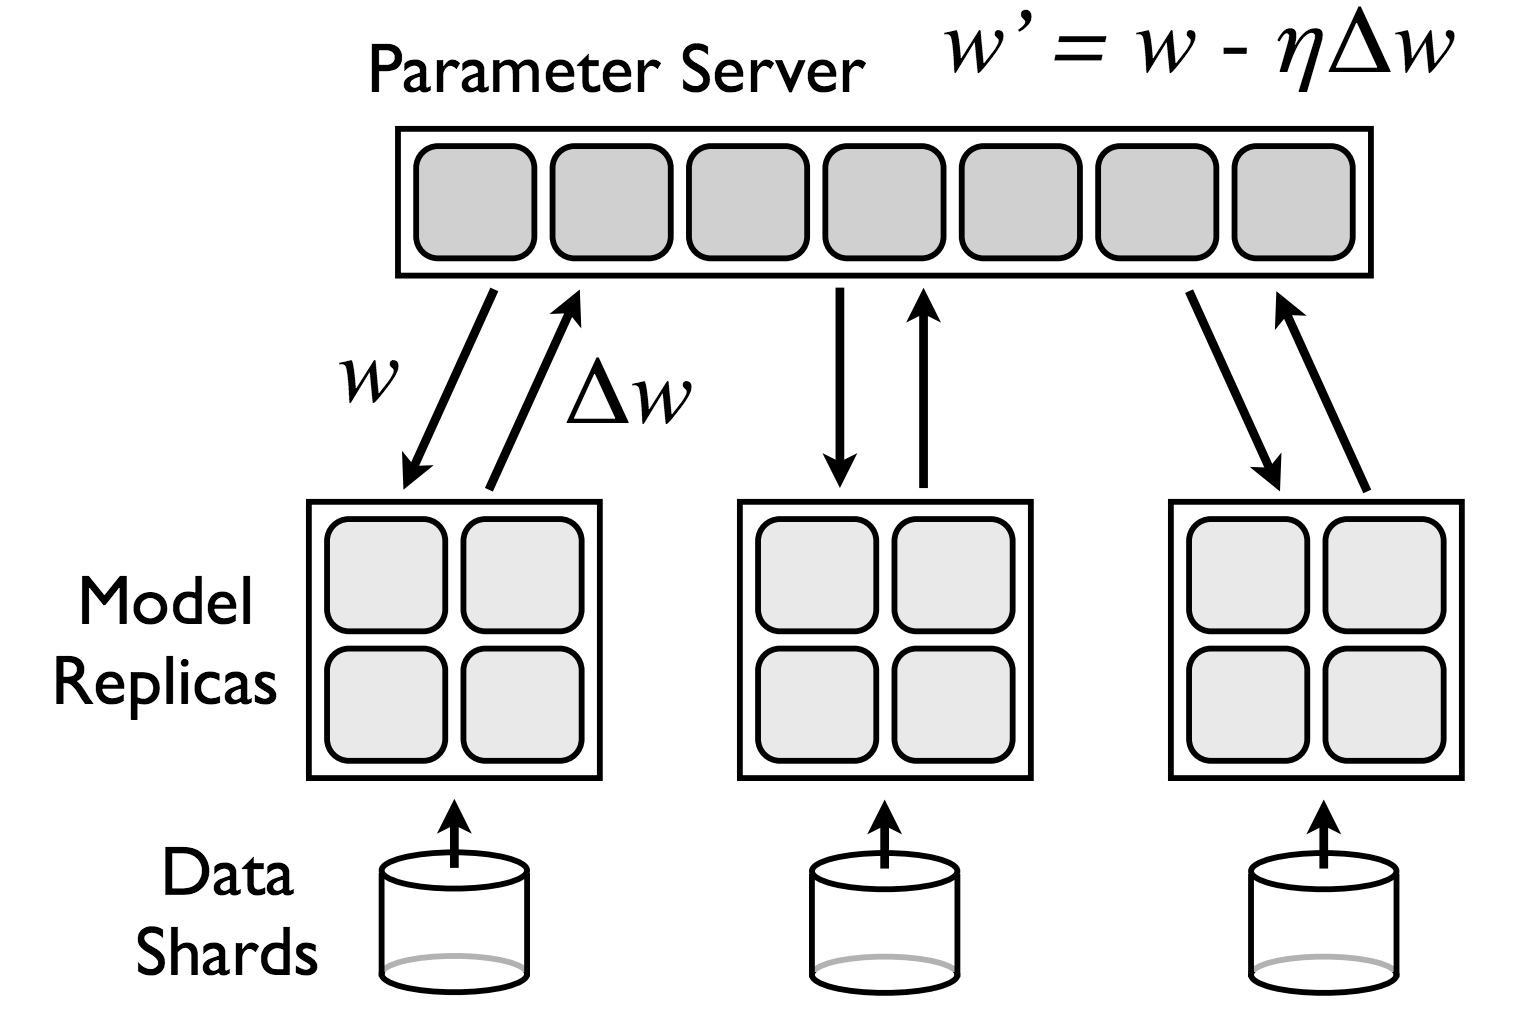
\includegraphics[scale=0.3]{./images/data_parallelism.png}
	\centering
	\caption{Data parallelism architecture performing Stochastic Gradient Descent (SGC). Model replicas at each node calculate gradients $\Delta w $ on a piece of data. Gradients are later transmitted asynchronously to Parameter Server to calculate updated weights.}
	\label{fig:data_parallelism}
\end{figure}
In a similar manner, in model parallelization scheme, models are cut into smaller pieces, which allows for scaling of the model. A drawback of model parallelization is that you have to synchronize all your copies of the model even more frequently than data parallelization. Synchronization should take place for each model at every layer of it, which for nowadays deep networks can be tens of layers. Thus, networking plays an very important role when it comes to model parallelization. For instance, a typical neural network architecture with 1 billion nodes may require tens of seconds is using a typical Ethernet networking for synchronization. As a results, HPC known tools such a Infiniband and PCI Express would greatly enhance the networking bottleneck for Inter-node and Intra-node communications respectively.\\
\begin{figure}[h]
	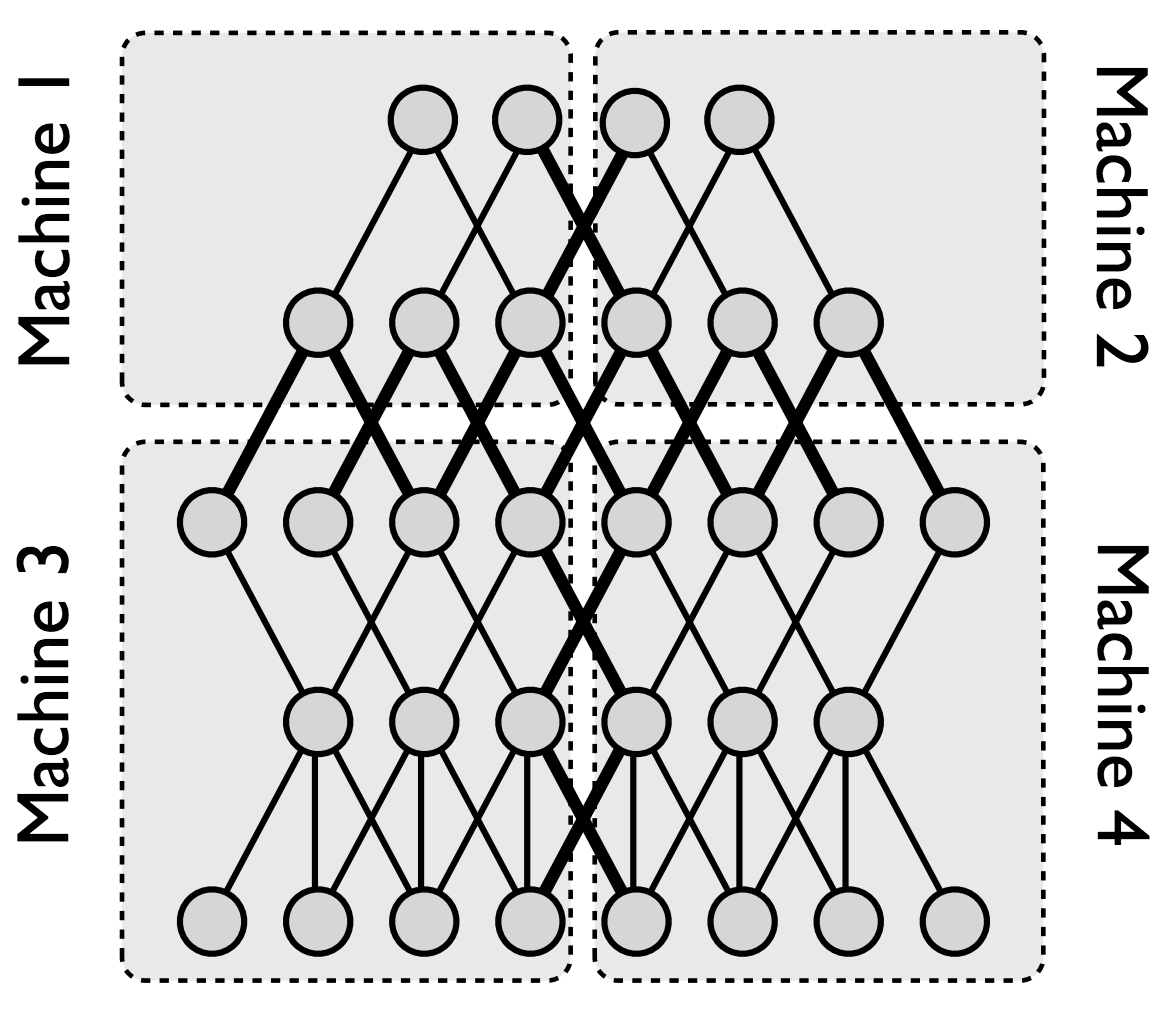
\includegraphics[scale=0.3]{./images/model_parallelism.png}
	\centering
	\caption{An example of model parallelism scheme in DistBelief framework for deep distributed neural networks by Google \cite{dean2012large}. Model is distributed accross four machines. Only nodes, which have edges crossing from one machine to another need to report their state.}
	\label{fig:model_parallelism}
\end{figure}

There are many primary questions to be addressed when thinking about integration of machine learning and HPC. Questions such as, aside from accelerating machine learning applications with GPUs and FPGAs, is traditional HPC ready to be the drive force behind data savvy machine learning applications? Are current top 500 supercomputers capable of powering new AI era of machine learning and deep learning? From software point of view, does conventional HPC require extensive modification to deal with mostly correlated data variables in machine learning application?
In the remaining of this section we will briefly introduce some of the ongoing researches and projects concentrated empowering machine learning with HPC medium.

\subsection*{Project Adam: Building an Efficient and Scalable Deep Learning Training System \cite{chilimbi2014project}}
In 2012 Google announced that they have trained an unsupervised image recognition neural network with 1 billion connections using 10 million training images, which can recognize cats from Youtube videos. Their training system consisted of a cluster of 1,000 computers with an aggregate of 16,000 cores \cite{le2013building}.\\

Project Adam by Microsoft could be thought as the successor of Google's project. The goal of the project Adam is to train a photograph classifier using 14 million images of Imagenet \cite{deng2009imagenet} into 22,000 image categories. The trained system by project Adam is claimed to be 50 times faster than the state of the art system. Speed is not the only concern of Microsoft researchers, it is also claimed that the system will be as twice accurate with 30 times less number of machines.\\

\subsection*{High level architecture}
Adam is similar in architecture to the Multi-Spert system introduced by Farber at Berkeley \cite{farber1997parallel}. A set of machine have the role of providing the inputs of the neural network with the input data, while another set train the model. Adam takes advantage of both model and data parallelism. Models are partitioned into many worker machines. Data is also fragmented to provide data parallelism. In order for each piece of the model to be trained only by a small chunk of data, many replicas of the same piece of model in parallel are trained on different data chunks.\\
\begin{figure}[h]
	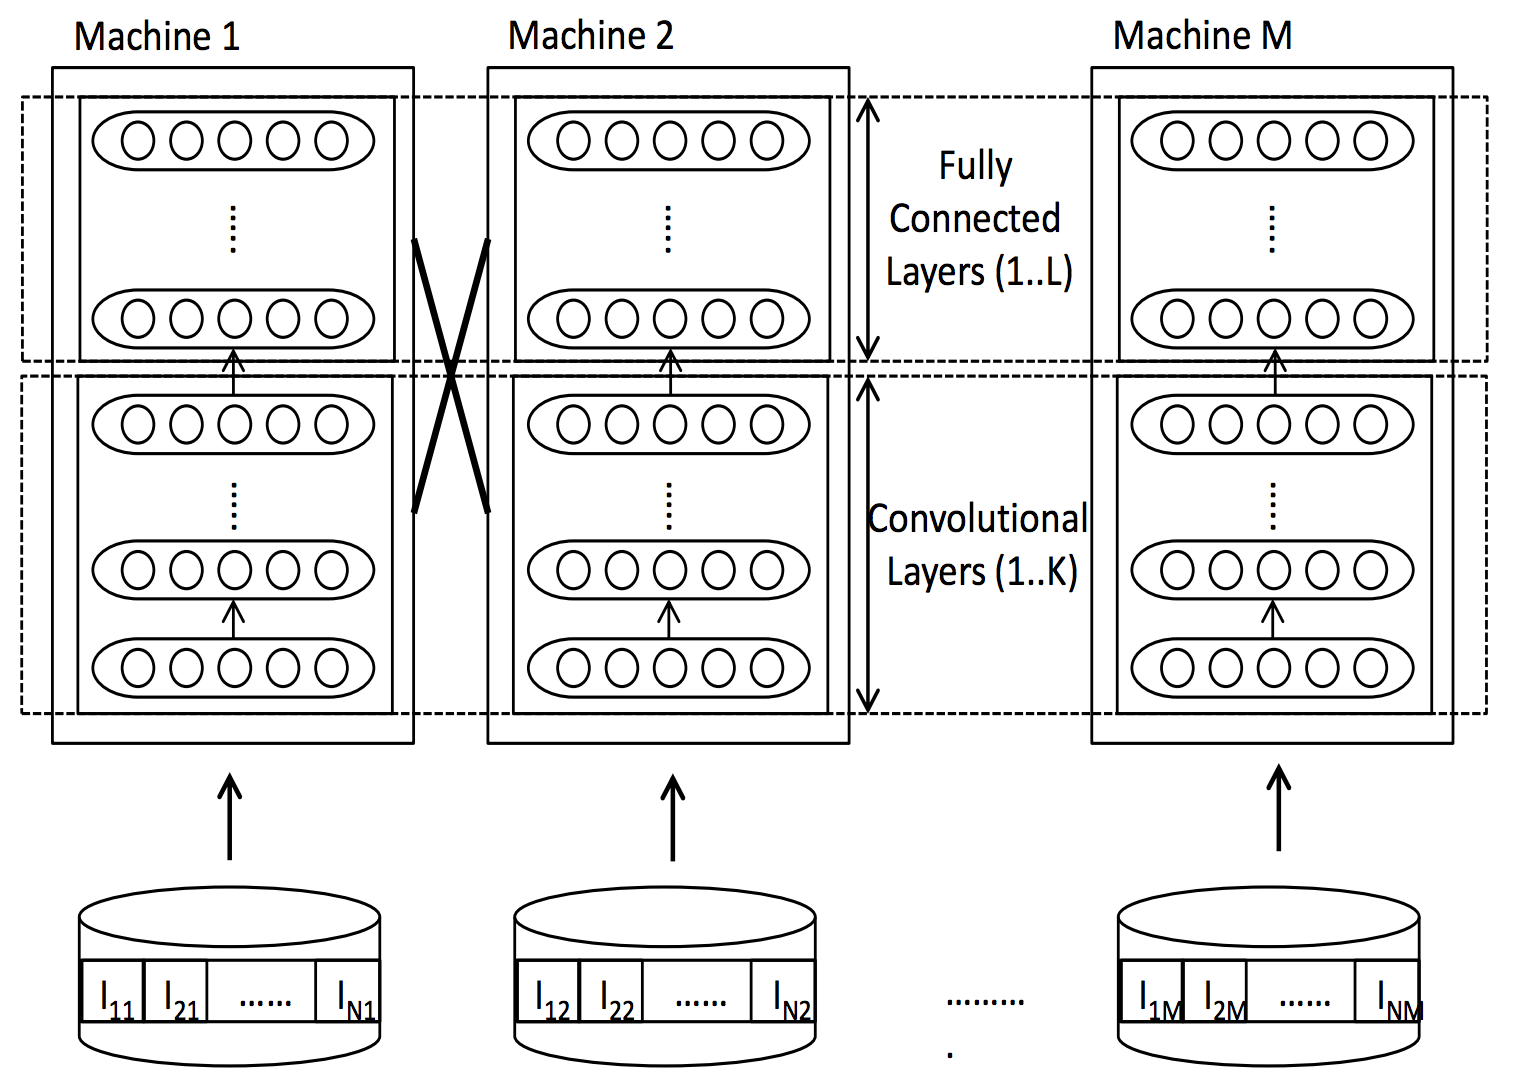
\includegraphics[scale=0.3]{./images/adam_parallelization.png}
	\centering
	\caption{Model and data partitioning in Adam architecture\cite{chilimbi2014project}.}
	\label{fig:adam_parallelism}
\end{figure}

A global Parameter Server stores the global values for the updated weights of all model pieces and replicas. The communication between the models and the Partition Server is asynchronous. Although the asynchrony between models and Parameter Servers may seem to introduce inconsistencies, but due to the resilient nature of the neural networks, they usually get trained successfully. As a matter of fact Microsoft researchers found that when they switched from asynchronous to synchronous communication between the models and the Parameter Server, the accuracy of the model dropped. The drop in the accuracy is justified as most of cost functions is datasets such as Imagenet and MNist are not convex functions. As a result, during the training process, the trainer may gets stuck at local optima rather than the global optima. The asynchronous updating of the weights cause the trainer in local optima get some momentum to escape local optima towards a global optima.\\

Convolutional neural networks are a special type of neural networks that has one or more convolution layers. Such networks are primary choice for image classification and vision since convolutional layers are capable of detecting features. It should be noted that Adam is not merely an image classification system and is capable of training any deep neural network with back-propagation. Figure \ref{fig:adam_parallelism} shows that Adam is partitioned in a way that each machine possess some of the convolution and some of the fully connected layers. This type partitioning allows for the communication of the convolution layers across machines be minimized.\\

\subsection*{Intra machine architecture and optimizations}

Training process on each single machine is multi-threaded. Threads hold activation functions and weights to use during feed-forward and back-propagation through None Uniform Memory Access (NUMA) fashion to reduce the cross-memory bus traffic.\\

Earlier we mentioned that neural networks are resilient so that we could use asynchronous communication between machines and global Parameter Server for updating weights. Same argument could be applied here for weight updates by threads on a single machine. On each machine a shared model holds the weights from all of threads weight updates. In order to avoid the lock times, threads update weights on the shared model without locking. Resilience of the neural networks along with commutativity and associativity properties of weight updates make the model work despite possible overwriting and race conditions of weight updates. This is one of the most important optimizations that allow scaling of deep neural network training process.\\

\subsection*{Memory optimizations}

During the training process weights need to be transmitted back and forth among layers. In order to minimize redundant copies, a pointer is passed along rather than rather than the values. In addition, in the model parallelism architectures, there are some communication between layers across multiple machines. These non-local communications are performed through a library built by project Adam team. The library is custom fit to the communication design of Adam, which supports pointer addressing to blocks of neurons that their output needs communication.\\

The partitioning of the models is Adam is done in a way that the working sets fit inside a L3 cache. Besides, an assembly kernel is implemented and tuned to exploit the locality during feed-forward and back propagation. The kernel allows for optimal matrix multiplication whether row major or column major blocks of weights are to be multiplied.\\

\subsection*{Global Parameter Server}

The Global Parameter Server holds the updated weights of the overall model from all machines. Due to high volume of weight updates, the Global Parameter Server of Adam require a more complex design rather than a conventional key value store. Figure \ref{fig:adam_global_param} depicts the architecture of the Global Server node for Adam.
\begin{figure}[h]
	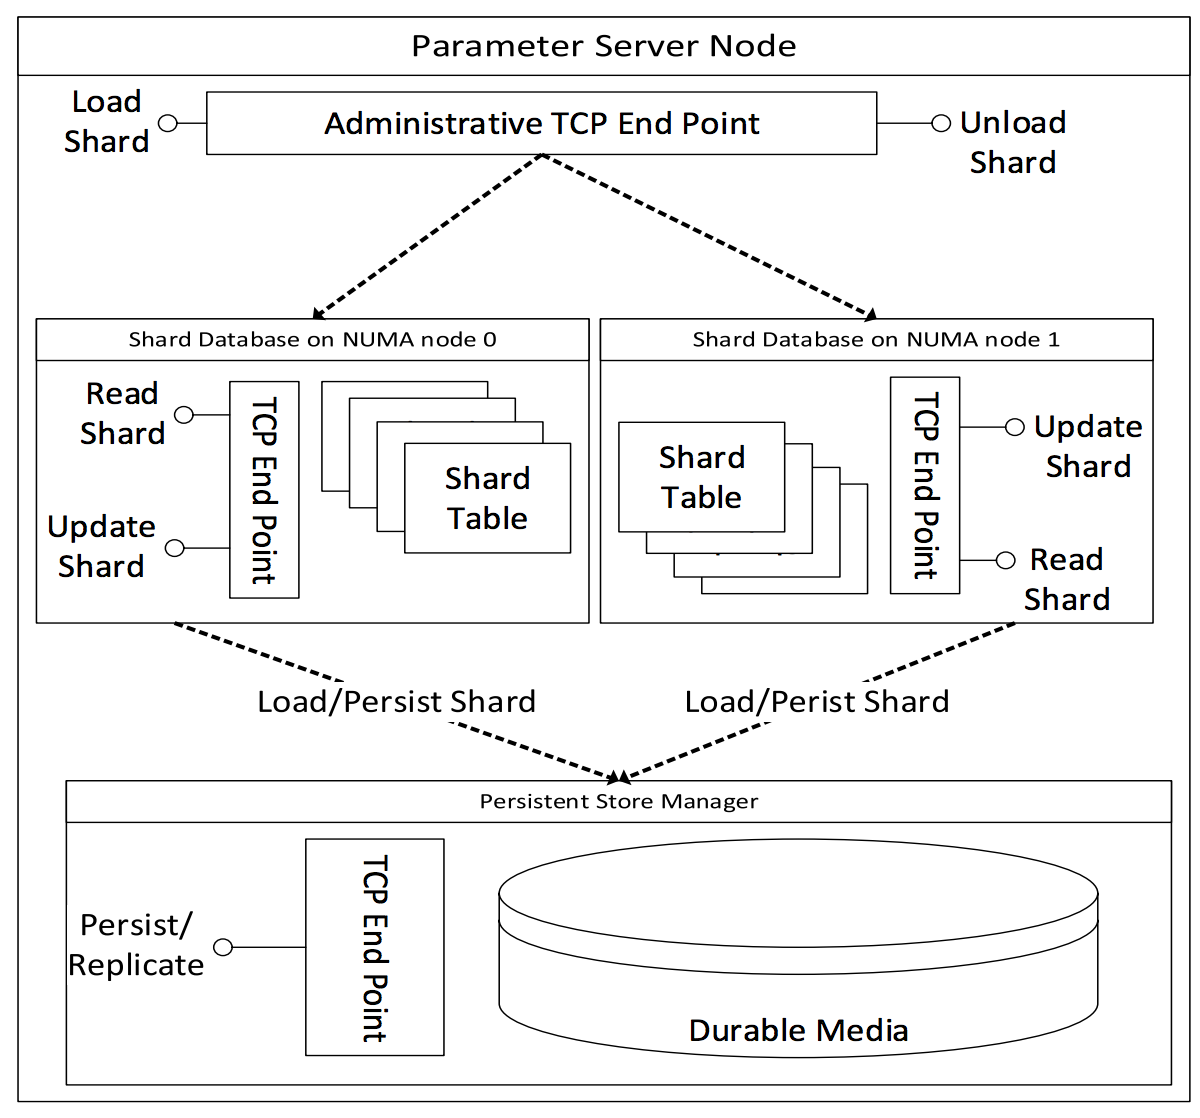
\includegraphics[scale=0.42]{./images/adam_global_param_server.png}
	\centering
	\caption{Global Parameter Server architecture of Adam\cite{chilimbi2014project}.}
	\label{fig:adam_global_param}
\end{figure}

Model parameters on the parameter server is partitioned into weight shards of size 1MB. The model partition in the Parameter Server helps with the spatial locality of the updates. In addition, to lower the communication between L3 caches and the parameter server, weight updates are not sent over to the parameter server once they are ready. Instead, weights are batched into blocks and then transferred over to parameter server. To assure the fault tolerance of the processes on the parameter server, there are three copies of weight shards available. One of the shards is assigned as the primary and the other two as the secondary to be used in the primary is cannot be used.

\subsection*{Project Adam's Hardware} Adam is formed of a cluster of 120 machines in three racks connected using IBM G8264 switches. Machine is Adam cluster are ervers of HP Proliant servers consisting of dual Intel Xeon E5-2450L processors with 16 cores and 98GB main memory along with two 10Gb NICs and one 1Gb NIC. There are four 7200 rpm hard drive storages for each machine. One of the hard drives that has the Windows 2012 server as operating server is of size 1TB. The rest three hard drives each are 3TB and are connected is RAID fashion. Out of 120 machines, 90 are allocated for training the model, 20 for parameter server, and the rest 10 for image inputs.

\subsection*{Results}

The accuracy of trained models is always one of the most important concerns. Adam's trained models are evaluated against two benchmarks. First, the MNIST benchmark that is well known to the machine learning community, which contains image of a series of handwritten digits. Second, the ImageNet, which is an image dataset with 22k object categories.\\

Adam architecture for testing against the MNIST benchmark consisted of two convolutional layers, two fully connected layers, and a ten class softmax output layer\cite{simard2003best}. The accuracy of Adam compared to the top 1  model by Goodfellow et al \cite{goodfellow2013maxout} is shown in table \ref{table:MNIST}.

\begin{table}
	\centering
	\caption{Adam accuracy on MNIST benchmark compared to the existing top accuracy model.}
	\begin{tabular}{ |p{5cm}|p{2cm}|  }
		\hline
		\textbf{Model} & \textbf{Accuracy} \\
		\hline
		Goodfellow et al. & 99.55\%\\
		\hline
		Adam (asynchronous) & 99.63\% \\
		\hline
		Adam (synchronous) & 99.39\% \\
		
		\hline
		
	\end{tabular}
	\label{table:MNIST}
\end{table}

It should be noted that the Adam accuracy is reported with asynchronous and synchronous communication of model shards in machine to the global parameter server. We mentioned that due to resiliency of the neural networks weight updates can be sent to global parameter server asynchronously. Even withing a machine weight updates coming from multiple threads is also asynchronous without using locks. The results in table \ref{table:MNIST} show that asynchrony not only did not lower the Adam accuracy, but also improved it by $0.24\%$.\\

For the ImageNet dataset, Adam was trained with a common architecture as reported in earlier works in literature. The architecture consist of 5 convolutional layers, 3 fully connected layers, and a 22k-way softmax layer. The accuracy of Adam compared to the top 1 system by Le et al \cite{le2013building} is tabulated table \ref{table:ImageNet}.

\begin{table}
	\centering
	\caption{Adam accuracy on ImageNet benchmark compared to the existing top accuracy model.}
	\begin{tabular}{ |p{5cm}|p{2cm}|  }
		\hline
		\textbf{Model} & \textbf{Accuracy} \\
		\hline
		Le et al. (without pre-training) & 13.6\%\\
		\hline
		Le et al. (with pre-training)  & 15.8\% \\
		\hline
		Adam & 29.8\% \\
		
		\hline
		
	\end{tabular}
	\label{table:ImageNet}
\end{table}

The results in table \ref{table:ImageNet} show a much more significant improvement by a factor of almost $2\times$ compared to the top accuracy model by Le et al \cite{le2013building}. The training process took 10 days to complete on a total of 62 machines, which is 32 times less than 2000 machines used by the top 1 model.\\

In conclusion, Adam succeeded to outperform the top 1 model in accuracy, number of machines used, and XXXX through a set of optimizations. It also seems that asynchrony plays a major role in enabling Adam to scale well training very large models.




\subsection*{Dadiannao: A machine-learning supercomputer \cite{chen2014dadiannao}}
With the re-emergence of neural networks in 2006 and introduction of deep learning algorithms, one stream of research has been focused on specialized hardware tailored to deep learning applications rather than using multi-purpose GPUs \cite{temam2012defect}\cite{esmaeilzadeh2012neural}.\\

One of such specialized deep learning accelerators is the one introduced by Chen et al, namely DianNao \cite{chen2014diannao}. DianNao comprises two major group of components. First, buffers for retrieving and holding inputs and outputs of neurons and synapses. Second, a Neural Functional Unit (NFU), which performs typical computations required to calculate outputs of neurons. These calculations are mainly matrix multiplication of weights and input in the first stage, summation of the results of first stage in the second stage, and applying an activation function in the third stage. Depending on the architecture of network and the layer types some other types of operation is also embedded such as convolution, averaging, etc. Figure \ref{fig:diannao_arch} depicts the block diagram of the DianNao accelerator.
\begin{figure}[h]
	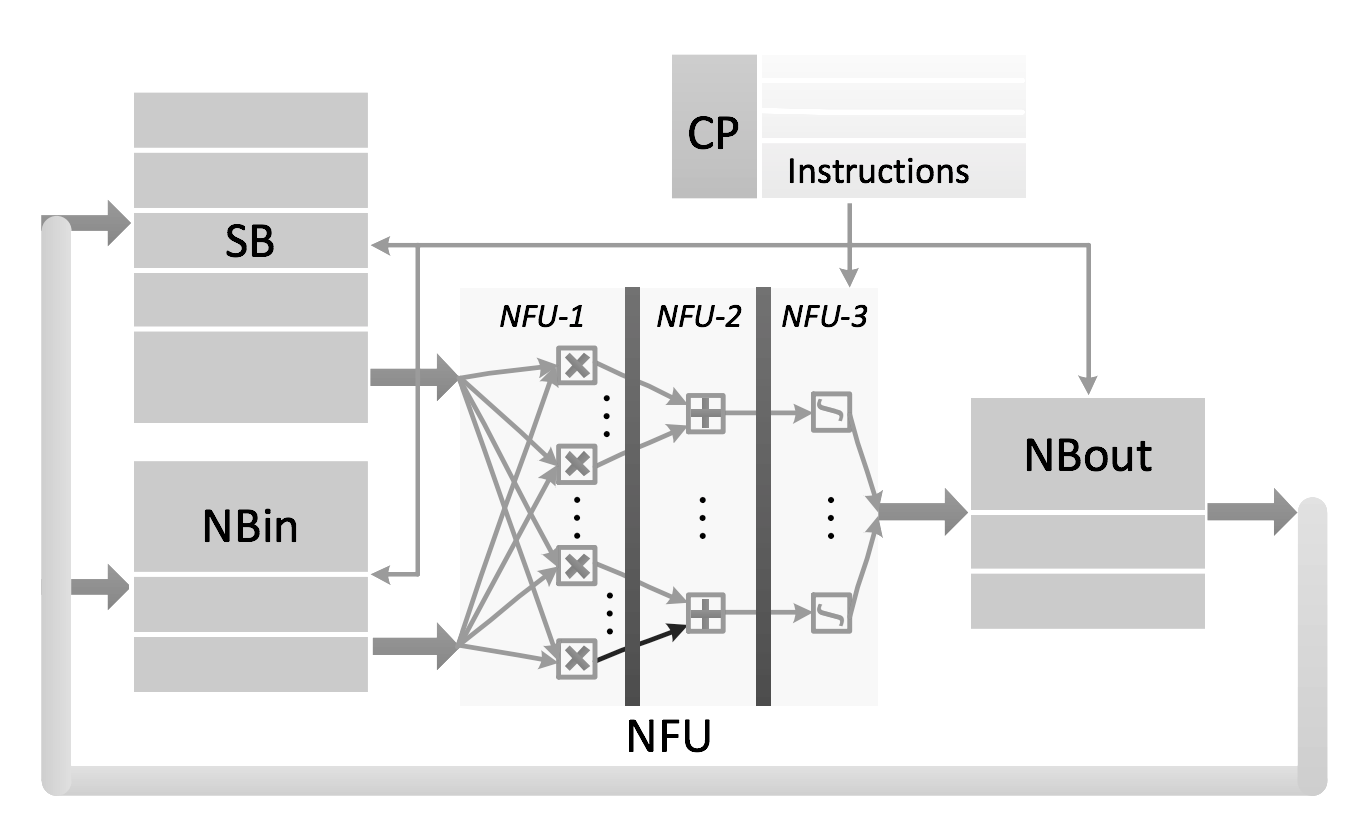
\includegraphics[scale=0.42]{./images/diannao.png}
	\centering
	\caption{Block diagram of the DianNao accelerator\cite{chen2014dadiannao}.}
	\label{fig:diannao_arch}
\end{figure}
In order to evaluate the performance of DianNao, Chen et al. structure two neural networks with similar architecture, but one with GPU and the other one with DianNao acceleration. They also implemented the same network using CPU only without any acceleration. Figure \ref{fig:diannao_speedup} compares the speedup of GPU over both DianNao and CPU.
\begin{figure}[h]
	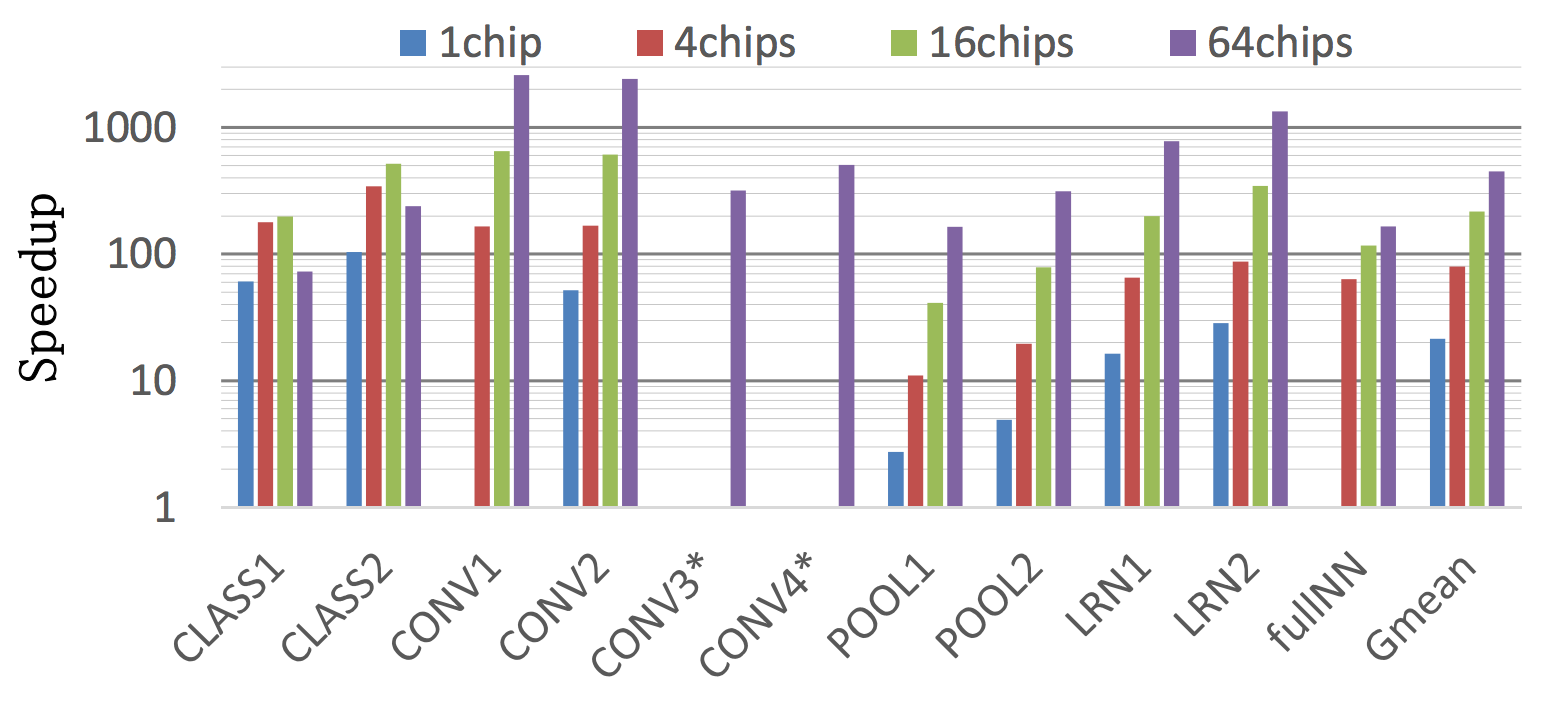
\includegraphics[scale=0.42]{./images/diannao_speedup.png}
	\centering
	\caption{Speedup of CPU/GPU and CPU/DianNao for various layer types of network\cite{chen2014dadiannao}.}
	\label{fig:diannao_speedup}
\end{figure}

We can see from figure \ref{fig:diannao_speedup} that DianNao give speedups up to 100 for some of the layers. However, in some other layers, mostly convolutional layers with private kernels and classification layers, which are common in both Deep Neural Networks (DNN) and Convolutional Neural Networks (CNN), GPUs may be preferred over DianNao. Authors believe that memory bandwidth is the major reason that DianNao performs worse than GPU in such layers. It should be noted that both convolutional and classification layers share the property that they have high number of synaptic connections even in range of millions. As DianNao takes up only about 53\% of the GPU (K20M), which is used for the sake of this comparison, it has the potential to compete GPUs.
\subsection*{Dadiannao, the machine learning supercomputer}

While the authors name Dadiannao the machine learning supercomputer, it seems the seems the design of Dadiannao were more focused on DNNs and CNNs. With that in mind, Dadiannao is capable of holding large models of even up to tens of GB in size in a multi node structure.\\

As we mentioned in the earlier part of this section, memory is thought to be the bottleneck of DianNao in convolutional layers with private kernel and classifier layers. The design of Dadiannao as a supercomputer aims to address these problems. First, in order to minimize data movement cost, synapses are placed near to the neurons consuming their data in a fully distributed architecture with no main memory unit. Secondly, nodes are biased towards storing data rather than computation. Thirdly, since the number of synaptic connections is orders of magnitude bigger than neurons,  instead of sending synaptic weights to neurons, neuron values is sent to synapses. This saves a lot in inter node communication bandwidth. Fourthly, intra-node, the storage units are broken into many storage units to increase the bandwidth.\\

The high level architecture of Dadiannao consist of many nodes arranged in a mesh configuration. Each node contains the storage units to store the synaptic and neuron values. In addition a, NFU unit is embedded similar to what introduced in DianNao \cite{chen2014diannao}.The NFU in Dadiannao is capable of carrying out more complex types of computation depending on the layers and mode of operation (training or inferencing). Figure \ref{fig:NFU_Diagram} shows the block diagram of a node for Dadiannao architecture. \\

\begin{figure}[h]
	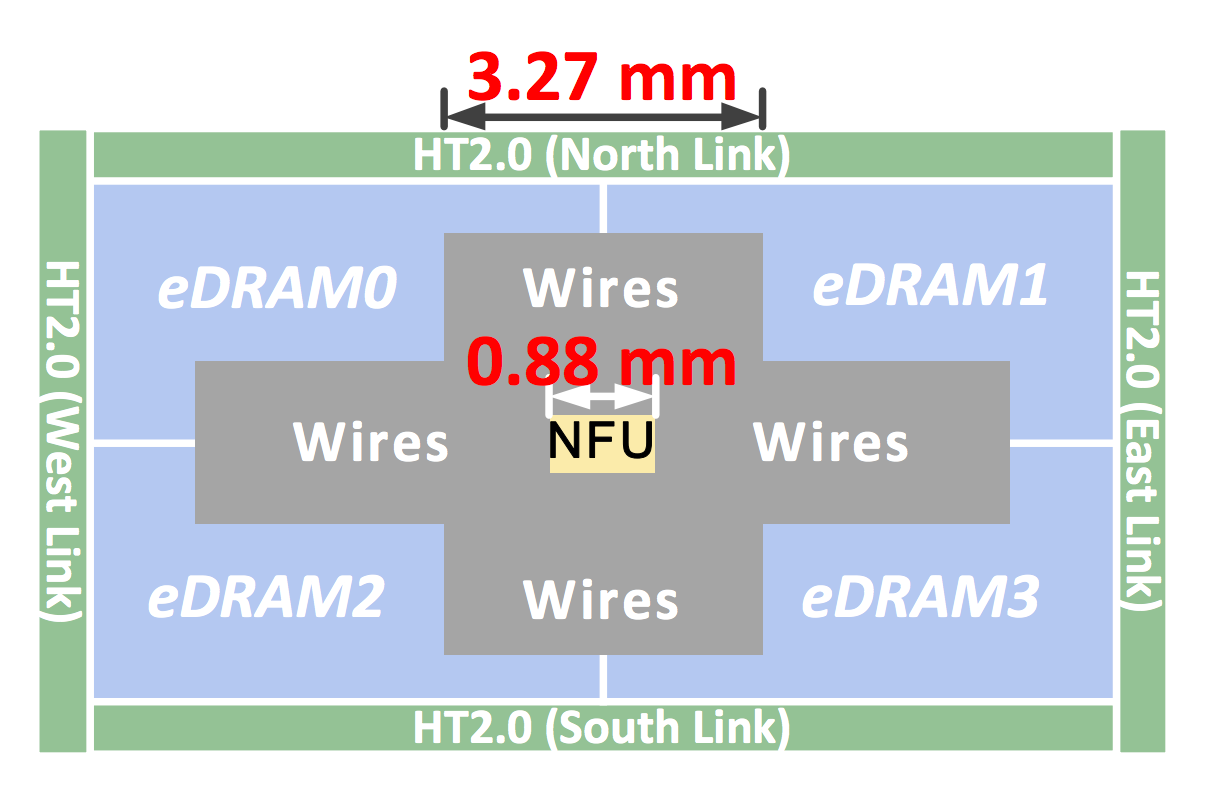
\includegraphics[scale=0.42]{./images/NFU_diagram.png}
	\centering
	\caption{Block diagram of a node within Dadiannao architecture \cite{chen2014dadiannao}.}
	\label{fig:NFU_Diagram}
\end{figure}
It should be noted that although SRAMs are generally preferred over other types of memory such as DRAM and eDRAM due to the higher speed, their size is limiting factor for them. A typical eDRAM can accommodate more than $2.5\times$ data compared to a SRAM. It should be noted that more storage density is required if parameters of big models are to be stored within chip to avoid external memory access. As a result, eDRAM is selected over SRAM in Dadiannao's proposed design. Refuting the memory bandwidth limitations for for computational units allows for scaling since more inputs and outputs to each neuron can be calculated simultaneously. However, eDRAMs suffer from some drawbacks compared to SRAMs namely, slower response, periodical refreshing requirement, and destructive read that may result in inaccurate values.\\

In order to exploit high bandwidth within nodes, a tile fashion layout is implemented as shown in figure \ref{fig:tiles}. In this design output neurons are assigned to various tile units. This enables NFUs to process data from multiple neurons in parallel.
\begin{figure}[h]
	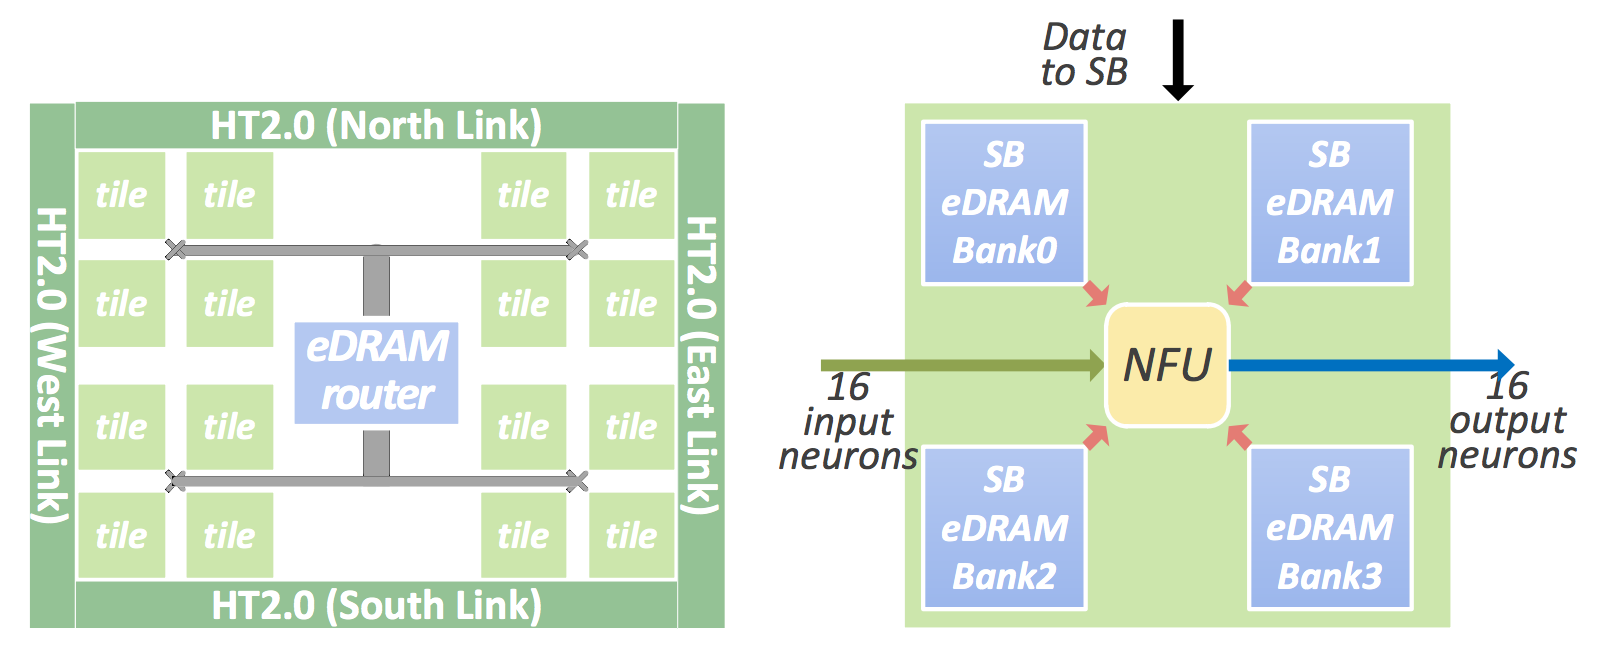
\includegraphics[scale=0.42]{./images/tiles.png}
	\centering
	\caption{Left: Tile implementation of a node. Right: Layout of unit inside a tile. \cite{chen2014dadiannao}.}
	\label{fig:tiles}
\end{figure}

Tiles in figure \ref{fig:tiles} are connected to two eDRAM reservoirs in the middle, one for input neurons from tiles and one for output neurons. It should be noted that even though there are many tiles and NFUs in a node, the number of neurons in a typical deep learning architecture is much more to be a one to one relationship between NFUs and neurons. As a result, each NFU has the job of calculating many neuron outputs. 

\subsection*{Experimental Results}
In this part we present the performance and energy consumption Dadiannao. In figure \ref{fig:diannao_speedup}, performance of Dadiannao in the training mode is compared against its NVIDIA K20M GPU implementation counterpart.
\begin{figure}[h]
	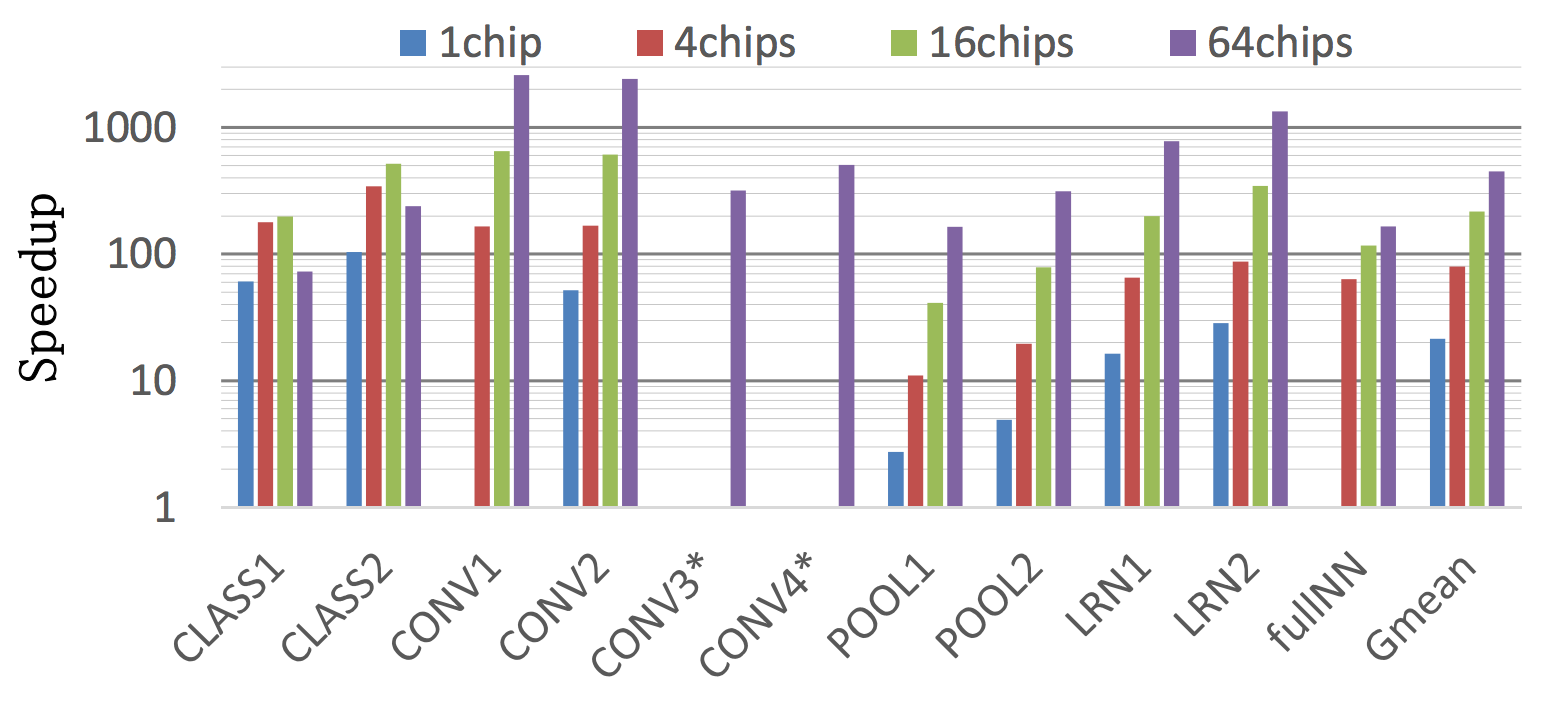
\includegraphics[scale=0.45]{./images/dadiannao_speedup.png}
	\centering
	\caption{Speedup of Dadiannao/GPU for various types of layers. CONV1 and fullNN layers require at least 4 nodes. CONV3* and CONV4* need at least 36 nodes to operate\cite{chen2014dadiannao}.}
	\label{fig:dadiannao_speedup}
\end{figure}

Figure \ref{fig:dadiannao_speedup} shows that Dadiannao could reach a speedup of more than 100 over the GPU system in almost all types of layers. The speedup is even higher up to more than 2000 for the CONV1 and CONV2 layers. It should be noted that the size of CONV3* and CONV4* layers (which have private kernels) is relatively large in the range of GB. As a result, the performance of these layers can only be measured of on a more than 36-node arrangement. The fullNN layer, which is a fully connected layer also accounts for more than 50M synaptic connections and hence cannot be implemented on a system with only 1 node. Generally speaking, average speedup of $21.38\times,$ $79.81\times,$ $216.72\times,$and $450.65\times$ is reported for Dadiannao over GPU for 1-node, 4-node, 16-node, and 64-node configurations, respectively. However, the speedup and scaling of various types of layers are wildly different due to the inherent characteristics of each type of layer.\\

Similarly, the performance of Dadiannao against GPU baseline in evaluated from energy point of view. Figures \ref{fig:dadiannao_training} and \ref{fig:dadiannao_inference} depict these performance analysis for both training and inference modes. In the training mode the energy reduction rates against the GPU baseline are $172.39\times,$ $180.42\times,$ $142.59\times,$ and $66.94\times$ for the 1-node, 4-node, 16-node, and 64-node respectively. The energy reduction number reported in the inference mode is even higher. In the inference mode, the energy reduction for the 1-node, 4-node, 16-node, and 64-node configuration is $330.56\times,$ $323.74\times,$ $270.04\times$, and $150.31\times,$ respectively.

\begin{figure}[!htb]
	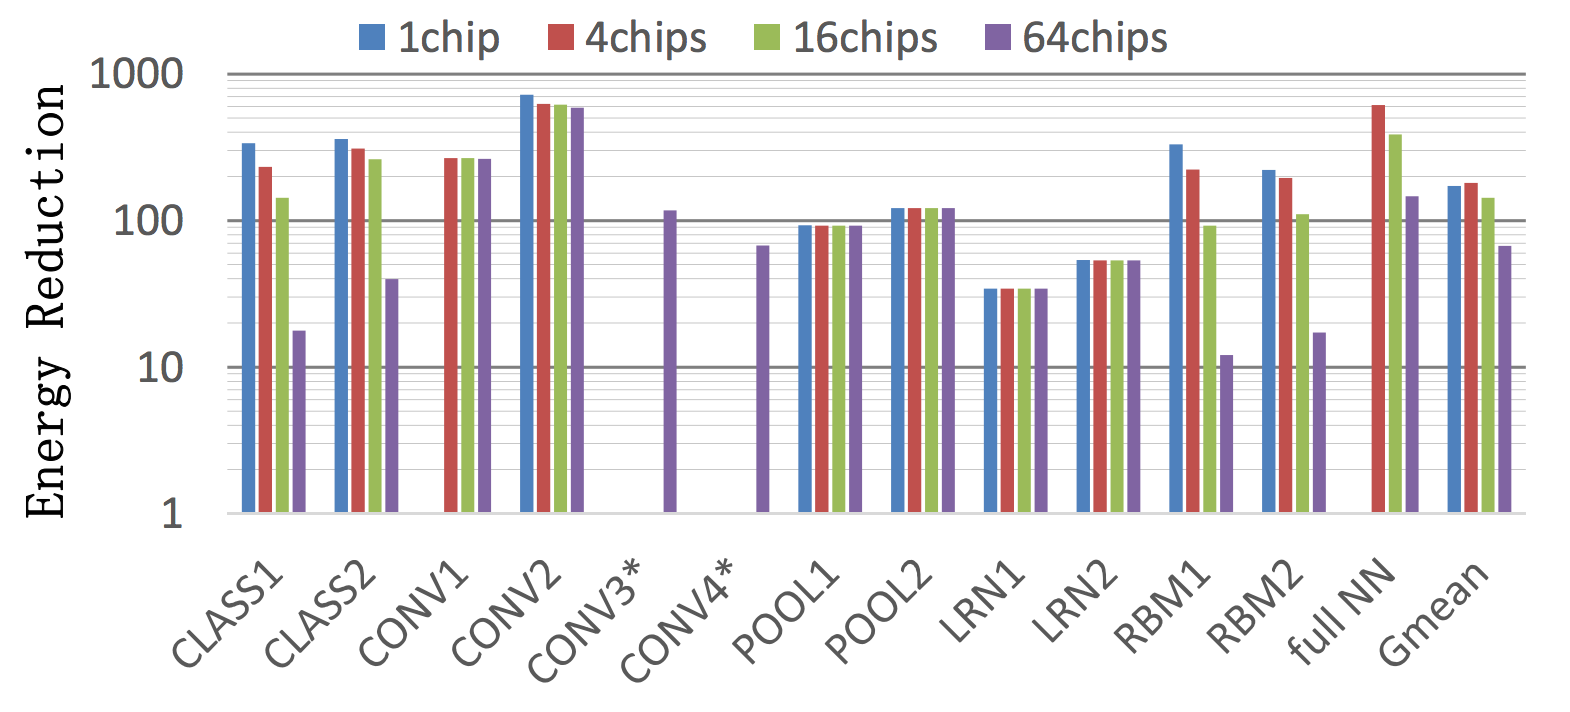
\includegraphics[scale=0.45]{./images/dadiannao_training.png}
	\centering
	\caption{Comparison of energy reduction of Dadiannao against GPU in the training mode\cite{chen2014dadiannao}.}
	\label{fig:dadiannao_training}
\end{figure}
\begin{figure}[!htb]
	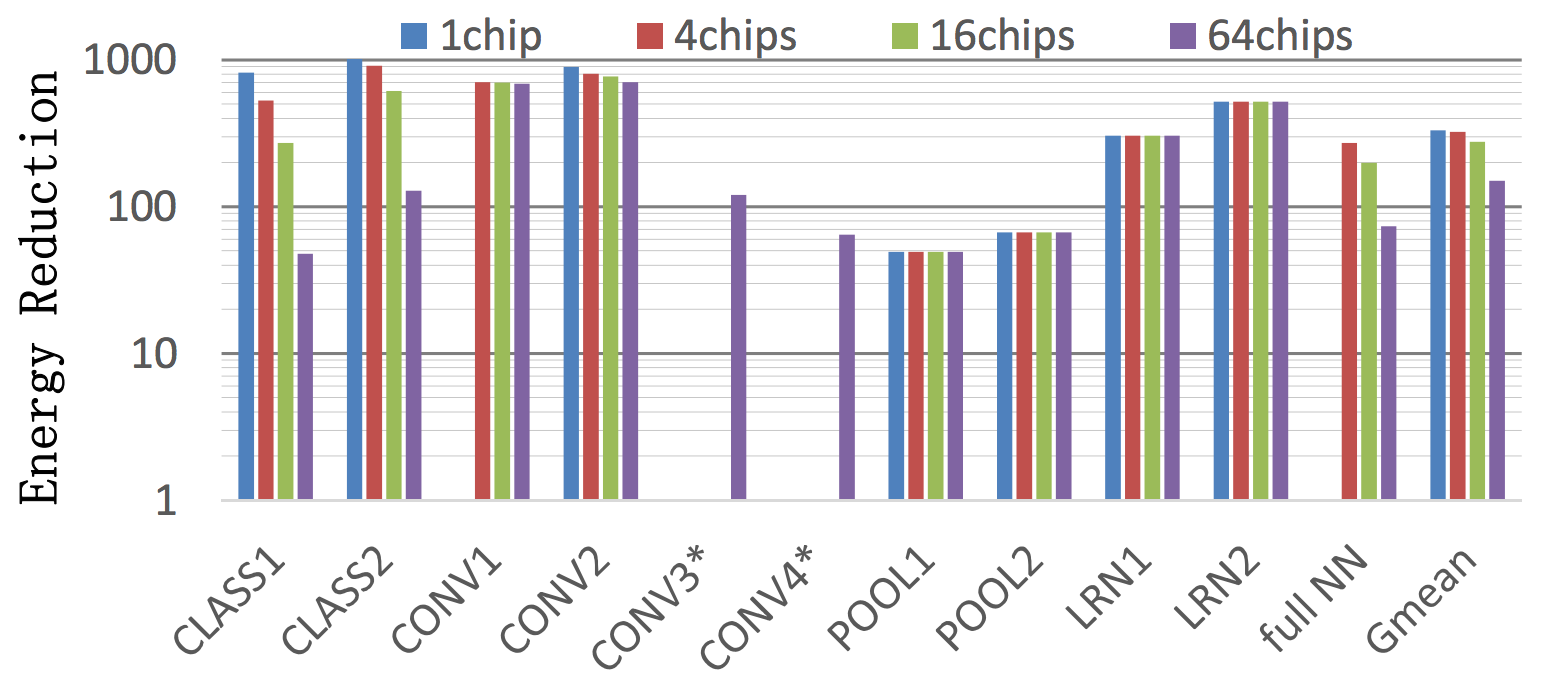
\includegraphics[scale=0.45]{./images/dadiannao_inference.png}
	\centering
	\caption{Comparison of energy reduction of Dadiannao against GPU in the inference mode\cite{chen2014dadiannao}.}
	\label{fig:dadiannao_inference}
\end{figure}

\section*{Conclusion and Outlook}
Machine learning and deep learning  have already become a part of our lives that we even do not notice them anymore. From search engines, voice recognition systems in our phones, and self-driving cars, all the way to commercial and financial analytics, they all benefit from machine learning and deep learning. With the help of fast CPUs and GPUs, training of models within machine learning and deep learning frame encountered a huge boost in the recent past. However, it seems that the future attempts to guarantee the the scalability of such systems should be focused on designing specialized software and hardware frameworks tailored to these applications such as project Adam by Microsoft and Dadiannao supercomputer. 

%%%%%%%%%%%%%%%%%%%%%%%%%%%%%%%%%%%%%%%%%%%%%%%%%%%%%%%%%%%%%%%%%%%%%%%%%%%%%%%
\bibliographystyle{splncs03}
\bibliography{paper_2.bib}

All links were last followed on October 5, 2014.
%%%%%%%%%%%%%%%%%%%%%%%%%%%%%%%%%%%%%%%%%%%%%%%%%%%%%%%%%%%%%%%%%%%%%%%%%%%%%%%
\nocite{*}
\end{document}
